\documentclass[border=3pt]{standalone}
% Shared preamble for every generated figure.
% Matches the report: newtx (Times), greyscale, square boxes.
\usepackage{newtxtext,newtxmath}
% newtx's typewriter (txtt) draws a slashed zero; use Latin Modern instead.
\renewcommand{\ttdefault}{lmtt}
\usepackage{tikz}
\usetikzlibrary{positioning,arrows.meta,calc,fit,backgrounds,shapes.geometric,
                decorations.pathreplacing,decorations.pathmorphing,matrix,patterns}

\definecolor{figgrey}{gray}{0.88}
\definecolor{figmid}{gray}{0.60}
\definecolor{figdark}{gray}{0.35}

\tikzset{
  fig/.style={font=\small},
  box/.style={draw,thick,minimum height=8mm,minimum width=22mm,align=center,
              inner sep=2pt,font=\small},
  greybox/.style={box,fill=figgrey},
  smallbox/.style={draw,minimum height=6mm,minimum width=16mm,align=center,
                   inner sep=2pt,font=\scriptsize},
  ln/.style={-{Stealth[length=2.2mm,width=1.8mm]},thick},
  lnb/.style={{Stealth[length=2.2mm,width=1.8mm]}-{Stealth[length=2.2mm,width=1.8mm]},thick},
  lbl/.style={font=\scriptsize,inner sep=1.5pt},
  note/.style={font=\scriptsize\itshape,inner sep=1.5pt},
}

\begin{document}
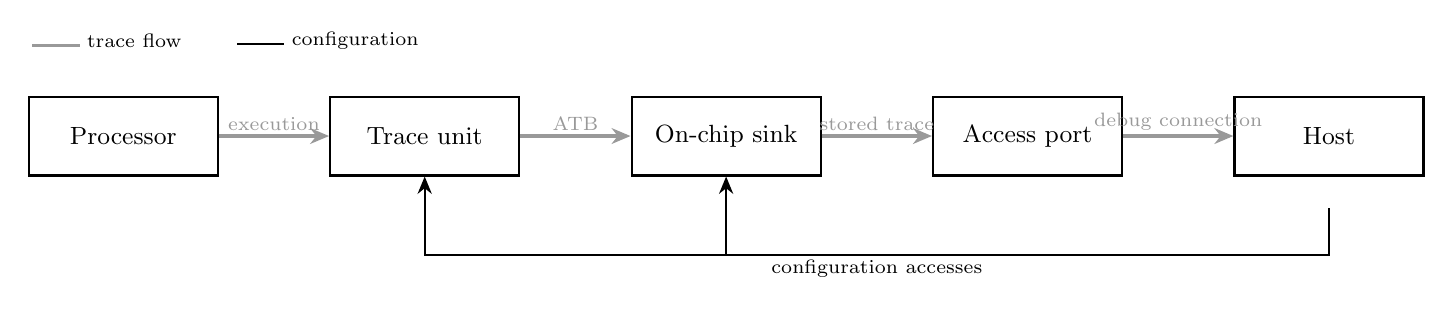
\begin{tikzpicture}[fig,
  cp/.style={draw,thick,minimum height=10mm,minimum width=24mm,align=center,font=\small},
  tr/.style={-{Stealth[length=2.4mm,width=2mm]},line width=1.3pt,figmid},
  cf/.style={-{Stealth[length=2.2mm,width=1.8mm]},thick}]

\node[cp] (cpu) {Processor};
\node[cp,right=14mm of cpu] (etm) {Trace unit};
\node[cp,right=14mm of etm] (tmc) {On-chip sink};
\node[cp,right=14mm of tmc] (ap)  {Access port};
\node[cp,right=14mm of ap]  (host){Host};

\draw[tr] (cpu) -- node[lbl,above]{execution} (etm);
\draw[tr] (etm) -- node[lbl,above]{ATB} (tmc);
\draw[tr] (tmc) -- node[lbl,above]{stored trace} (ap);
\draw[tr] (ap)  -- node[lbl,above]{debug connection} (host);

\draw[cf] ($(host.south)-(0,4mm)$) -- ++(0,-6mm) -| node[lbl,pos=0.25,below]{configuration accesses} ($(etm.south)-(0,0mm)$);
\draw[cf] ($(host.south)-(0,10mm)$) -| ($(tmc.south)-(0,0mm)$);

\node[lbl,anchor=west] at ($(cpu.north west)+(0,7mm)$) {\textcolor{figmid}{\rule{6mm}{1.1pt}}\ trace flow};
\node[lbl,anchor=west] at ($(cpu.north west)+(26mm,7mm)$) {\rule{6mm}{0.8pt}\ configuration};

\end{tikzpicture}
\end{document}
